\documentclass[esd, manuscript]{copernicus} % uncomment to see what the 2 column final paper will look like.

\begin{document}

\begin{figure}[t]
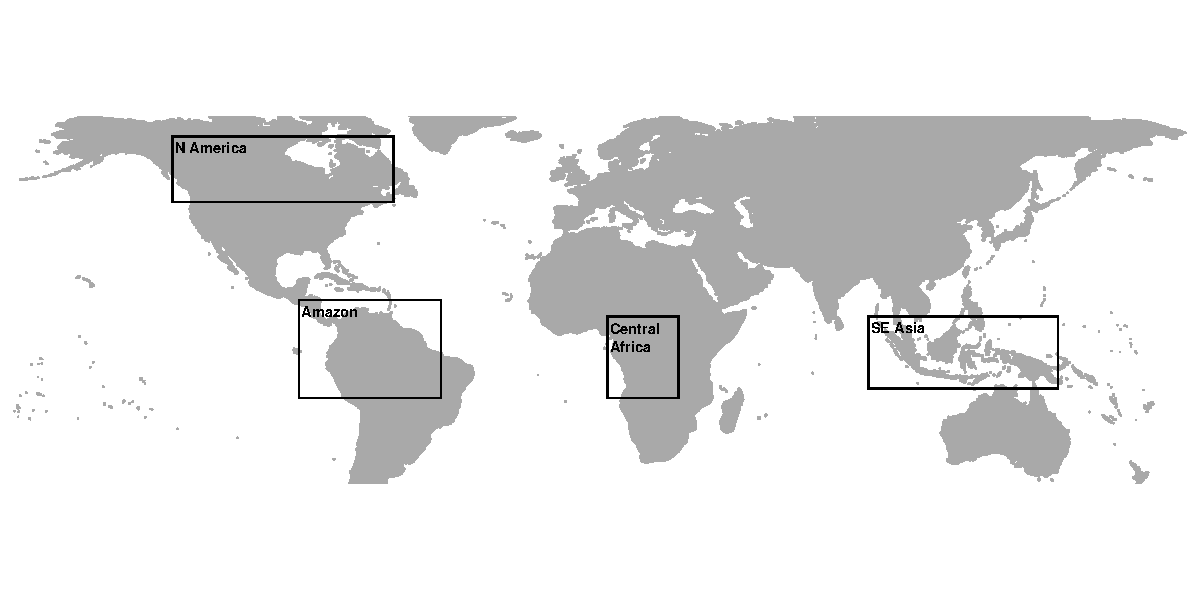
\includegraphics[width=12cm]{graphics/map_forests.pdf}
\caption{A map of the forest regions used in the study. Regions are: Amazon 15\textdegree S - 15\textdegree N, 270\textdegree E - 315\textdegree E; Central Africa; 15\textdegree S - 10\textdegree N, 7.5\textdegree E - 30\textdegree E; SE Asia 12\textdegree S - 10\textdegree N, 90\textdegree E - 150\textdegree E; North America 45\textdegree N - 65\textdegree N, 230\textdegree E - 300\textdegree E.}
\label{fig:map_forests}
\end{figure}

\begin{figure}[t]
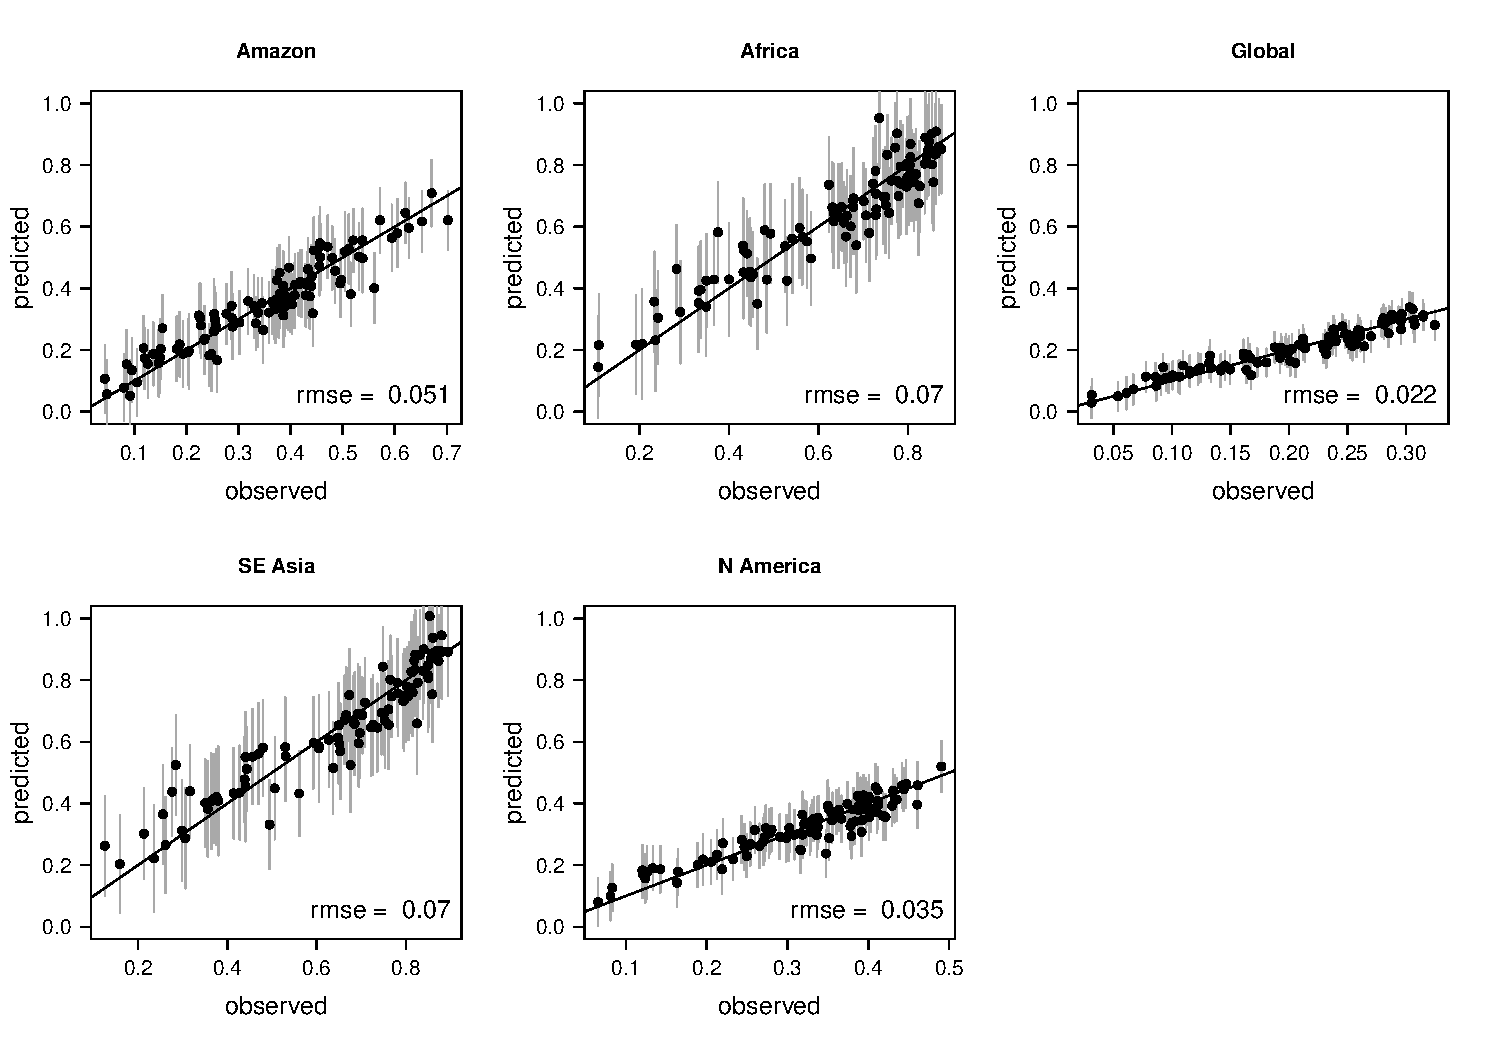
\includegraphics[width=12cm]{graphics/frac_loo.pdf}
\caption{Leave-one-out cross validation performance of the emulator, when reproducing each forest fraction. Black points represent the emulator central estimate of a held-out point, with grey lines representing $\pm$ 2 standard deviations.}
\label{fig:frac_loo}
\end{figure}

\end{document}